\documentclass[12pt]{article}

\usepackage[margin=1in]{geometry}
\usepackage{amsmath,amsthm,amssymb}
\usepackage{mathrsfs}
\usepackage{mathtools}
\usepackage{enumitem}
\usepackage{physics}

\usepackage{pdfpages}

\newcommand{\magsq}[1]{\big|#1\big|^2}
\newcommand{\avg}[1]{\left<#1\right>}
\newcommand{\fullint}{\int_{-\infty}^\infty}
\newcommand{\fullintd}[1]{\fullint\dd#1\:}
\newcommand{\cint}[2]{\int_{#1}^{#2}}
\newcommand{\cintd}[3]{\cint{#1}{#2}\dd#3\:}
\newcommand{\e}{\mathbf{e}}

\begin{document}
	
\title{Homework 1}
\author{Sean Ericson \\ Phys 684}
\maketitle

\section*{Problem 1}
We can get the electric field amplitude from the intensity, as
\[ I = \frac{P}{A} = \frac{1}{2}c\epsilon_0E_0^2 \implies E_0 = \sqrt{\frac{2P}{c\epsilon_0A}} \approx 868\text{ V/m}.\]
A rough but simple estimate for the dipole moment is just $e a_0 \approx 2.5$ Debye. The Rabi frequency is then
\[ \Omega_0 = \frac{\mu E_0}{\hbar} \approx 70\text{ MHz} \]
See the end of the document for a printout of the Mathematica notebook used for these calculations.

\section*{Problem 2}
Under the rotating wave approximation, we neglect the counter-rotating term and get as our differential equation (neglecting bars on the `c's)
\begin{align*}
    \dot{c}_1 &= -\frac{1}{2}i\Omega_0e^{i\delta t}c_2 \\
    \dot{c}_2 &= -\frac{1}{2}i\Omega_0e^{-i\delta t}c_1.
\end{align*}

The Rabi frequency is directly proportional to the applied electric field. In the weak-field limit, we can perturbatively expand the amplitudes as
\[ c_i = c_i^{(0)} + \Omega_0 c_i^{(1)} + \Omega_0^2 c_i^{(2)} + \cdots. \]

To zero-th order, the amplitudes are given by the initial conditions $c_1^{(0)} = c_1(0) = 1$, and $c_2^{(0)} = c_2(0) = 0$. Now we go to first order and plug into the differential equation:
\begin{alignat*}{3}
    &\quad & \dv{t}\left(c_1^{(0)} + \Omega_0c_1^{(1)}\right) &= -\frac{i}{2}\Omega_0e^{i\delta t}\left(c_2^{0} + \Omega_0c_2^{(1)}\right) \\
    &\implies\quad & \Omega_0\dot{c}_1^{(1)} &= -\frac{i}{2}\Omega_0^2e^{i\delta t}c_2^{(1)}
\end{alignat*}
Matching terms proportional to $\Omega_0$ gives
\begin{alignat*}{3}
    &\quad & \dot{c}_1^{(1)} &= 0 \\
    &\implies\quad & c_1^{(1)} &= c_1^{(1)}(0) = 0.
\end{alignat*}
For $c_2$, we find
\begin{alignat*}{3}
    &\quad & \dv{t}\left(c_2^{(0)} + \Omega_0c_2^{(1)}\right) &= -\frac{i}{2}\Omega_0e^{-i\delta t}\left(c_1^{(0)} + \Omega_0c_1^{(1)}\right) \\
    &\implies\quad & \Omega_0\dot{c}_2^{(1)} &= -\frac{i}{2}\Omega_0e^{-i\delta t} + O(\Omega^2) \\
    &\implies\quad & c_2^{(1)} &= -\frac{i}{2}\int_0^t\dd t' e^{-i\delta t'} \\
    & & &= \frac{1}{2\delta}\left(e^{-i\delta t} - 1\right).
\end{alignat*}

So, to first order we have that
\begin{equation*}
    \begin{rcases*}
        c_1 \approx 1 \\
        c_2 \approx \frac{\Omega_0}{2\delta}\left(e^{-i\delta t} - 1\right)
    \end{rcases*}
    \implies
    \begin{aligned}
        \magsq{c_1} &\approx 1 \\
        \magsq{c_2} &\approx \frac{\Omega_0^2}{2\delta^2}\left(1 - \cos\delta t\right)
    \end{aligned}
\end{equation*}


Repeating the process for second order (matching terms proportional to $\Omega_0^2$),
\begin{alignat*}{3}
    &\quad & \dv{t}\left(1 + \Omega_0^2 c_1^{(2)}\right) &= -\frac{i}{2}\Omega_0e^{i\delta t}\frac{\Omega_0}{2\delta}\left(e^{-i\delta}-1\right) \\
    &\implies\quad & \dot{c}_1^{(2)} &= -\frac{i}{4\delta}\left(1 - e^{i\delta t}\right) \\
    &\implies\quad & c_1^{(2)} &= -\frac{i}{4\delta}\int_0^t \dd t'\left(1 - e^{i\delta t}\right) \\
    & & &= -\frac{i}{4\delta}\left[t - \frac{1}{i\delta}\left(e^{i\delta t} - 1\right)\right]
\end{alignat*}
\begin{alignat*}{3}
    &\quad & \dv{t}\left(\frac{\Omega_0}{2\delta}\left(e^{-i\delta t} - 1\right) + \Omega_0^2c_2^{(2)}\right) &= -\frac{i}{2}\Omega_0e^{-i\delta t}\left(1 + \Omega_0^2 c_1^{(2)}\right) \\
    &\implies\quad & \dot{c}_2^{(2)} &= 0 \\
    &\implies\quad & c_2^{(2)} &= 0
\end{alignat*}

So, to second order we have
\begin{equation*}
    \begin{aligned}
        c_1 &\approx 1 - \frac{i\Omega_0^2}{4\delta}\left[t - \frac{1}{i\delta}\left(e^{i\delta t} - 1\right)\right] \\
        c_2 &\approx \frac{\Omega_0}{2\delta}\left(e^{-i\delta t} - 1\right)
    \end{aligned}
\end{equation*}
\begin{equation*}
    \implies
    \begin{cases*}
        \magsq{c_1} \approx 1 - \frac{\Omega_0^2}{2\delta}\left(1 - \cos\delta t\right) + \frac{\Omega_0^4}{8\delta^4}\left(1 + \frac{t^2}{2\delta^2} - \cos\delta t - 2t\sin\delta t\right)  \\
        \magsq{c_2} \approx \frac{\Omega_0^2}{2\delta^2}\left(1 - \cos\delta t\right)
    \end{cases*}
\end{equation*}

Now, for third order,
\begin{alignat*}{3}
    &\quad & \Omega_0^3\dot{c}_1^{(3)} &= -\frac{i}{2}\Omega_0e^{i\delta t}\left(\frac{\Omega_0}{2\delta}\left(e^{-i\delta t} - 1\right)\right) \\
    &\implies\quad & \dot{c}_1^{(3)} &= 0 \\
    &\implies\quad & \dot{c}_1^{(3)} & = 0
\end{alignat*}
\begin{alignat*}{3}
    &\quad & \Omega_0^3\dot{c}_2^{(3)} &= -\frac{i}{2}\Omega_0e^{-i\delta t}\left(1 - \frac{i\Omega_0^2}{4\delta}\left[t - \frac{1}{i\delta}\left(e^{i\delta t} - 1\right)\right]\right) \\
    &\implies\quad & \dot{c}_2^{(3)} &= -\frac{1}{8\delta}\left[t - \frac{1}{i\delta}\left(e^{i\delta t} - 1\right)\right] \\
    &\implies\quad & c_2^{(3)} &= -\frac{1}{16\delta^3}\left[2\left(e^{i\delta t} - 1\right) + \delta t (\delta t - 2i)\right].
\end{alignat*}

So, to third order
\begin{equation*}
    \begin{aligned}
        c_1 &\approx 1 - \frac{i\Omega_0^2}{4\delta}\left[t - \frac{1}{i\delta}\left(e^{i\delta t} - 1\right)\right] \\
        c_2 &\approx \frac{\Omega_0}{2\delta}\left(e^{-i\delta t} - 1\right) - \frac{\Omega_0^3}{16\delta^3}\left[2\left(e^{i\delta t} - 1\right) + \delta t (\delta t - 2i)\right]
    \end{aligned}
\end{equation*}
\begin{equation*}
    \implies
    \begin{cases*}
        \magsq{c_1} \approx 1 - \frac{\Omega_0^2}{2\delta}\left(1 - \cos\delta t\right) + \frac{\Omega_0^4}{8\delta^4}\left(1 + \frac{t^2}{2\delta^2} - \cos\delta t - 2t\sin\delta t\right)  \\
        \magsq{c_2} \approx \frac{\Omega_0^2}{2\delta^2}\left(1 - \cos\delta t\right) - 
    \end{cases*}
\end{equation*}



\section*{Problem 3}
\begin{enumerate}[label=(\alph*)]
    \item We consider a two-level atom with states denoted $\ket{1}$, $\ket{2}$ and corresponding energies $E_1 = \hbar\omega_1 = -\omega_0/2$ and $E_2 = \hbar\omega_2 = \omega_0/2$. The atom interacts with a linearly polarized optical field described by
    \[ \vec{E} = \Re[E_0e^{-i\omega t}]\;\hat{z}. \]
    The interaction between the atom and the field is given to lowest order by the electric dipole interaction
    \[ V = -\vec{\mu}\cdot\vec{E} = e z \abs{E_0}\cos(\omega t - \phi). \]
    Assuming the two atomic states have opposite parity, the diagonal interaction matrix elements vanish:
    \[ V_{11} \propto \mel{1}{z}{1} = 0 = V_{22}. \]
    By a choice of phase for the wavefunction, we can take the off-diagonal elements to be real (and hence equal):
    \[ V_{12} = e\abs{E_0}z_{12}\cos(\omega t - \phi) \]
    The hamiltonian for the combined system is then
    \begin{align*}
        H &= H_0 + V \\
        &= \frac{\hbar \omega_0}{2}\mqty(-1&0\\0&1) + \hbar\Omega_0\cos(\omega t - \phi)\mqty(0&1\\1&0) \\
        &= -\frac{\hbar\omega_0}{2}\sigma_z + \hbar\Omega_0\cos(\omega t - \phi)\sigma_x,
    \end{align*}
    where we define the Rabi frequency $\Omega_0 = \frac{ez_{12}E_0}{\hbar}$.

    In the Schr{\"o}dinger representation, the state of the atom is described by
    \[ \ket{\psi(t)}_\text{S} = c_1(t)\ket{1} + c_2(t)\ket{2} \quad \left(\magsq{c_1} + \magsq{c_2} = 1\right). \]
    In the absence of the external field, the state would evolve as
    \[ \ket{\psi(t)}_\text{S} = c_1(0)e^{-i\omega_1t}\ket{1} + c_2(0)e^{-i\omega_2t}\ket{2}. \]
    In the interaction representation, we factor out this free phase evolution by writing
    \[ \ket{\psi(t)}_\text{I} = \bar{c}_1(t)e^{-i\omega_1t}\ket{1} + \bar{c}_2(t)e^{-i\omega_2t}\ket{2}, \]
    that is, we make the (time-dependent) unitary transformation
    \[ \ket{\psi(t)}_\text{S} \to \ket{\psi(t)}_\text{I} = U(t)\ket{\psi(t)}_\text{S}, \]
    where
    \[ U(t) = \mqty(e^{-i\omega_1t}&0\\0&e^{-i\omega_2t}). \] 
    We get the effective interaction hamiltonian by making the inverse transformation on $V$:
    \[ V_\text{I} = U^\dag VU = \hbar\Omega_0 \cos(\omega t) \mqty(0&e^{-i\omega_0t}\\e^{i\omega_0t}&0), \]
    where the phase $\phi$ has been absorbed into the (complex) Rabi frequency.

    \item To make the rotating wave approximation, we re-write the effective hamiltonian as
    \begin{align*}
        V_\text{I} &= \frac{1}{2}\hbar\Omega_0\left(e^{i\omega t} + e^{-i\omega t}\right)e^{i\omega_0 t}\sigma_+ + \text{h.c.} \\
        &= \frac{1}{2}\hbar\Omega_0\left(e^{i(\omega + \omega_0)t} + e^{-i(\omega - \omega_0)t}\right)\sigma_+ + \text{h.c.}
    \end{align*}
    where $\sigma_+$ is the raising operator $\dyad{2}{1}$. Making the RWA amounts to neglecting the counter-rotating term (i.e. the term with $\omega_0 + \omega$), leaving
    \[ V_\text{I} \approx \frac{1}{2}\hbar\Omega_0e^{i\delta t}\sigma_+ + \text{h.c.}, \]
    where we have switched to using the detuning $\delta = \omega_0 - \omega$.

    \item The Bloch Siegert shift effectively decreases $\omega_2 - \omega_1 = \omega_0$, and therefore becomes relevant when the level spacing is already small, such as in magnetic field interactions.
\end{enumerate}

\section*{Problem 4}
Making the simplifying assumptions of a constant Rabi frequency and zero detuning, we have that
\begin{equation*}
    \begin{rcases*}
        \dot{c}_1 = -\frac{i}{2}\Omega_0c_2 -\frac{\gamma_1}{2}c_1 \\
        \dot{c}_2 = -\frac{i}{2}\Omega_0c_1 - \frac{\gamma_2}{2}
    \end{rcases*}
    \implies \mqty(\dot{c}_1\\\dot{c}_2) = -\frac{1}{2}\mqty(\gamma_1&i\Omega_0\\i\Omega_0&\gamma_2)\mqty(c_1\\c_2),
\end{equation*}
or, more simply,
\[ \dot{\psi} = M\psi; \qquad M = -\frac{1}{2}\mqty(\gamma_1&i\Omega_0\\i\Omega_0&\gamma_2). \]
For $c_1(0) = 1,\;c_2(0)=0$, the solution to this first order differential equation is
\begin{align*}
    \psi(t) &= e^{Mt}\psi(0) \\
    &= \frac{1}{2\chi} \mqty(e^{-(\gamma_1 + \gamma_2 + \chi)t}\left[\chi\left(e^{\chi t/2} + 1\right) + (\gamma_1 + \gamma_2)\left(e^{\chi t/2} - 1\right)\right] \\ -2ie^{-(\gamma_1 + \gamma_2 + \chi)/4}\left(e^{\chi t/2} - 1\right) )
\end{align*}

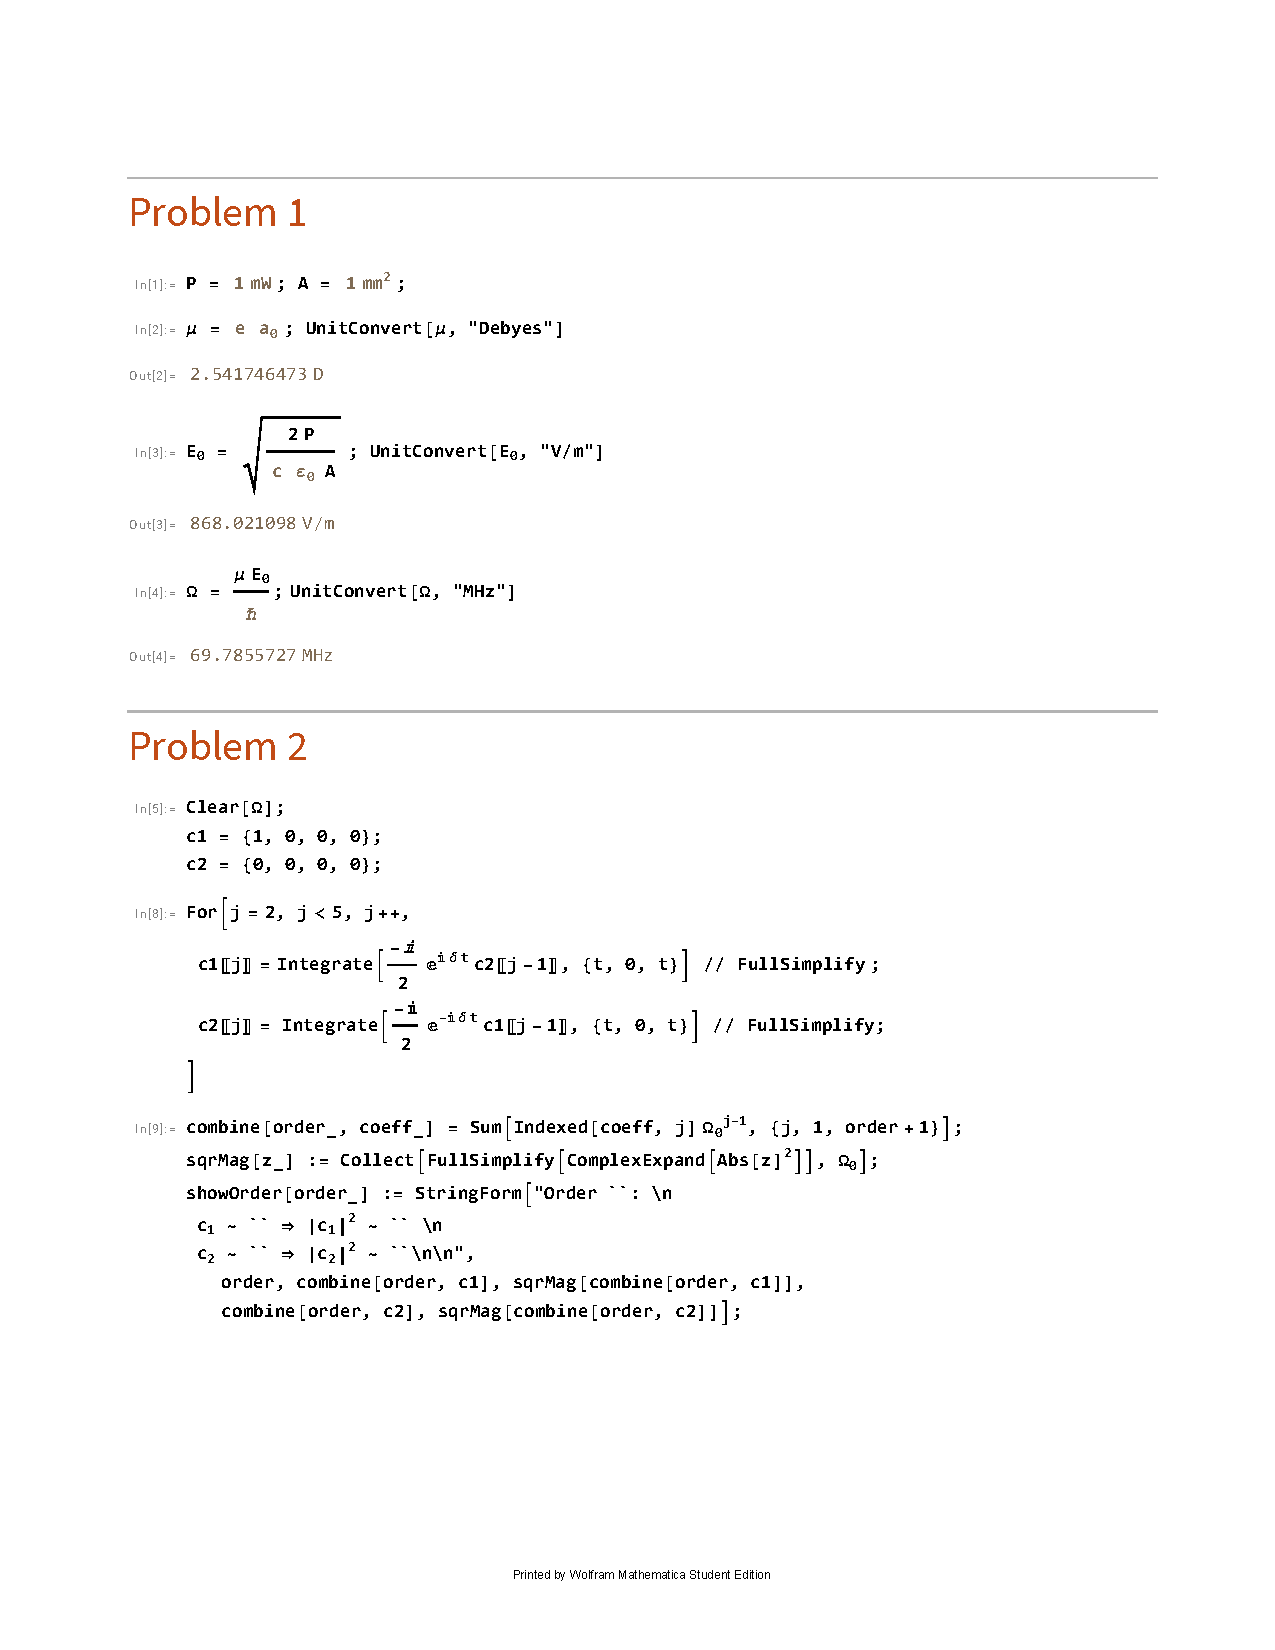
\includepdf[pages=-]{calcs/HW1_mathematica.pdf}
\end{document}